\section{Turbulence III}
Today we discuss turbulence in 2D. Under some conditions, we can approximate the Earth's atmosphere as a thin layer of fluid, or we can consider a fluid interface etc. To this end, we start by studying turbulence in 2D systems.

\subsection{Vorticity and Enstrophy}
Recall the Enstrophy\footnote{``I just had a rant that we don't use $Z$ (the partition function) in the class, but now it's back.... revenge of the $Z$''}:
\begin{equation}
    Z = \int d^d\v{x}(\nabla \times \v{v})^2
\end{equation}
with $d = 2$ and $\nabla \cdot \v{v} = 0$ (incompressability). The curl of the velocity field is the vorticity:
\begin{equation}
    \gv{\omega} = \nabla \times \v{v}
\end{equation}
Writing down the Navier-Stokes equation:
\begin{equation}
    \p_t \v{v} + \v{v} \cdot \nabla \v{v} = -\frac{1}{\rho}\nabla p + \nu \nabla^2\v{v}
\end{equation}
Now taking the curl of this equation (the pressure term drops out as the curl of a gradient is zero):
\begin{equation}
    \p_t \gv{\omega} + \nabla \times (\v{v} \cdot \nabla \v{v}) = \nu \nabla^2 \gv{\omega}
\end{equation}
To work on the second term, we consider the identity:
\begin{equation}
    \nabla(\v{u} \cdot \v{v}) = (\v{u} \cdot \nabla)\v{v} + (\v{v} \cdot \nabla)\v{u} + \v{u} \times (\nabla \times \v{v}) + \v{v}\times (\nabla \times \v{u})
\end{equation}
and in particular taking $\v{u} = \v{v}$:
\begin{equation}
    \nabla(\frac{1}{2}\abs{\v{v}}^2) = \v{v} \cdot \nabla \v{v} + \v{v} \times (\nabla \times \v{v})
\end{equation}
Thus:
\begin{equation}
    \nabla \times (\v{v} \cdot \nabla \v{v}) = \nabla \times (\nabla\left(\frac{v^2}{2}\right)) - \nabla \times (\v{v} \times \gv{\omega}) = \nabla \times (\gv{\omega} \times \v{v})
\end{equation}
where we have used again that the curl of a gradient is zero. Expanding out this last term:
\begin{equation}
    \nabla \times (\v{v} \cdot \nabla \v{v}) = (\v{v} \cdot \nabla)\gv{\omega} - (\gv{\omega}\cdot\nabla)\v{v} + \gv{\omega}(\nabla \cdot \v{v}) + \v{v}(\nabla \cdot \gv{\omega})
\end{equation}
The third term drops out because we assume the fluid is incompressible. The fourth term drops out because the divergence of a curl ($\gv{\omega}$ is a curl of $\v{v}$) is zero. Hence:
\begin{equation}
    \nabla \times (\v{v} \cdot \nabla \v{v}) = (\v{v} \cdot \nabla)\gv{\omega} - (\gv{\omega}\cdot\nabla)\v{v}
\end{equation}
So the Navier Stokes equation becomes:
\begin{equation}
    \p_t \gv{\omega} + (\v{v} \cdot \nabla)\gv{\omega} = (\gv{\omega} \cdot \nabla)\v{v} + \nu\nabla^2\gv{\omega}
\end{equation}
The object on the LHS is a total derivative, so let us write it this way. Further, for any 2D system, $\gv{\omega}$ points out of the plane while $\nabla$ exists in the plane, so $\gv{\omega}\cdot\nabla = 0$. Hence:
\begin{equation}
    \dod{\gv{\omega}}{t} = \nu \nabla^2\gv{\omega}
\end{equation}
Further, if we take the limit where the viscosity vanishes (e.g. the inertial range of the turbulent cascade), then:
\begin{equation}
    \dod{\gv{\omega}}{t} = 0
\end{equation}
Hence under our set of assumptions, $\gv{\omega}$ is conserved! The only way to not conserve it is to switch on a dissipation $\nu$. Any function of $\gv{\omega}$ is conserved, and hence $\gv{\omega}^2$ - the entstrophy density, and the total enstrophy, are both conserved. So in 2D, in addition to the energy, the enstrophy is also a conserved quantity. The question then becomes - can we have turbulent cascades in this setting? What are the consequences of conservation?

\subsection{Turbulence in 2D - Dual Cascade}
We can write the energy per unit area as:
\begin{equation}
    E = \frac{\text{Energy}}{\text{Area}} = \frac{1}{2}\avg{\v{v}^2} = \int E(k)dk
\end{equation}
we can write down an analogous expression for the enstrophy:
\begin{equation}
    Z = \frac{\text{Enstrophy}}{\text{Area}} = \frac{1}{2}\avg{\gv{\omega}^2} = \int k^2E(k)dk
\end{equation}
where we got the last expression by recalling that $\gv{\omega} = \nabla \times \v{v}$ and so $\gv{\omega}_\v{\v{k}} = i\v{k} \times \v{v}_{\v{k}}$. We can also look at the dissipated power:
\begin{equation}
    P = \nu \int d^d\v{x}(\p_i v_j)^2 \stackrel{\text{FT}}{\to} \nu k^2E(k)
\end{equation}

Now we ask - how do $E, Z$ cascade? They show a dual cascade behaviour, as shown by Fjørtoft in 1953. In $k$-space, the spectral density of $Z$ is related to the energy spectrum via $Z_k = k^2E(k)$ as we found above. Fjørtoft invites us to consider the following setup. We inject energy at $k_f$, in a band of size $\Delta_f$. In this range $\text{Re} \gg 1$ so no dissipation can occur. We consider a small and large $k_{d_1}, k_{d_2}$ where dissipation can occur. In between is the inertial range.

\begin{center}
    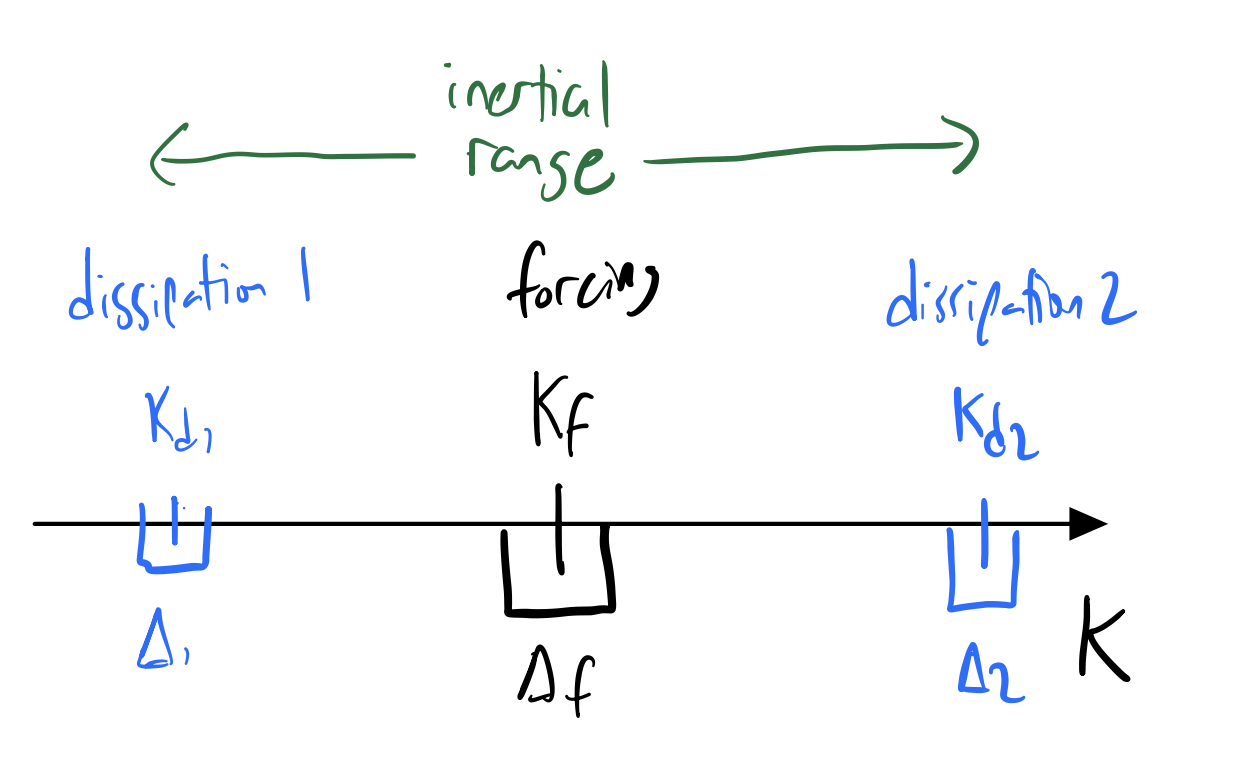
\includegraphics[scale=0.35]{Lectures/Images/lec14-kscale.png}
\end{center}

\begin{enumerate}
    \item Let us suppose that in range $\Delta_f$ around $k_f$ we produce energy per unit time of $\e$. This amounts to a respective rate of enstrophy production:
    \begin{equation}
        \eta = k_f^2\e
    \end{equation}
    \item Now, we construct a \emph{reductio ad absurdum}/proof by contradiction. Suppose now that a comparable amount of energy $\e$ is dissipated per unit time near $k_{d_2}$. This corresponds to a respective rate of enstrophy dissipation:
    \begin{equation}
        \eta' = k_{d_2}^2\e \gg k_f^2\e = \eta
    \end{equation}
    This is not possible in a steady state (i.e. it is not possible to dissipate $Z$ as a rate larger than the rate of production, as enstrophy is conserved). Thus we conclude most of the energy must be dissipated at the other end of the spectrum, near $k_{{d_1}}$.
    \item Similarly, assuming dissipation of $Z$ near $k_{d_1}$ at a rate $\eta$ also leads to a contradiction, as we dissipate $E$ at a rate:
    \begin{equation}
        \e' = \left(\frac{1}{k_{d_1}}\right)^2\eta \gg \left(\frac{1}{k_f}\right)^2\eta = \e
    \end{equation}
    \textcolor{red}{(Partially missed this part, so this argument may not quite be correct. I also didn't quite get the punchline of what we conclude from the proofs of contradiction.)}
\end{enumerate}

\begin{center}
    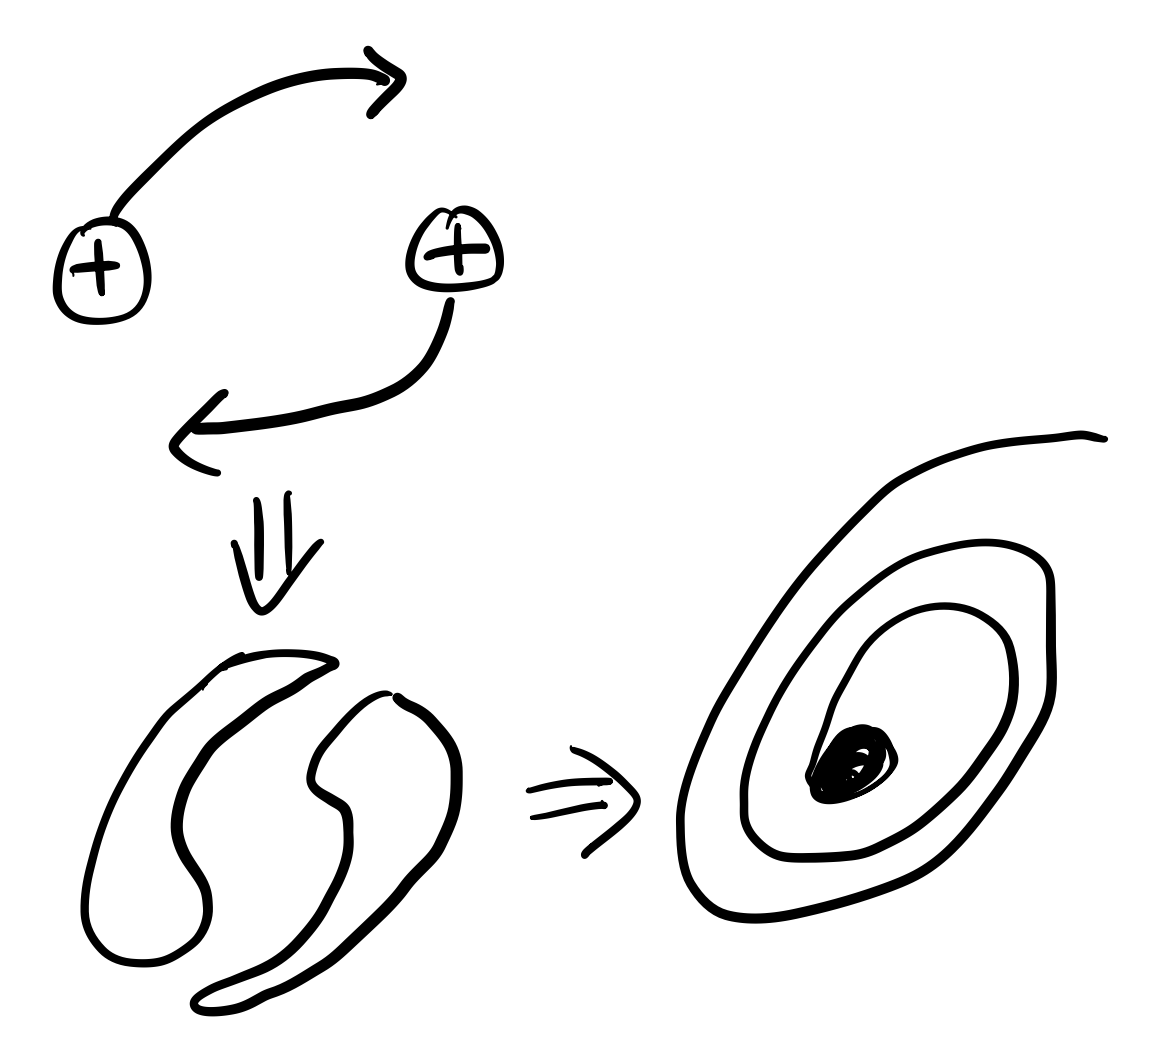
\includegraphics[scale=0.35]{Lectures/Images/lec14-vortexmerger.png}
\end{center}

What happens is we have 2D vortex mergers (two vortices of scale $L$ go to scale $2L$), where energy goes into the vortex core, while enstrophy goes into thin filaments. Simultaneously to this, there is a direct cascade of the enstrophy. This is the notion of the dual cascade in real space - concentration of enstrophy in the filaments, and the concentration of energy in the large-scale vortex cores.

What we will do next time - using the same dimensional analysis argument (a la Kolmogorov) we did in 3D to find the power spectrum in 2D. Since the enstrophy density has a $k^2$, we will see that it has a different power law. Then, we will see how even in 3D under the presence of odd viscosity we have quasi-2dimensionalization.